\documentclass[a4paper, 11pt]{article}

\usepackage[utf8]{inputenc}
\usepackage[english]{babel}

\usepackage{hyperref}

\usepackage{graphicx}
\usepackage{float}

\usepackage{fullpage}

\begin{document}
	\begin{centering}
		\large\textbf{Progress Report: 21/12/2016}\\
		~\\
		Oussama ENNAFII:
		\normalsize MATIS | TITANE \\
		Directors: Cl\'ement Mallet \& Florent Lafarge \\
	\end{centering}


	\section*{Data:}
	
	\begin{itemize}
		\item Available data:
			\begin{itemize}
				\item[-] Bati3D data mostly in 3DS format on: Aix, Annecy, Elancourt, Lambesc, Lyon, Montpellier, Nantes, Paris and Toulouse;
			\end{itemize}
		\item Ordered data:
			\begin{itemize}
				\item[-] BD Ortho (HR) on the same regions: Aix, Annecy, Elancourt, Lambesc, Lyon and Nantes;
			\end{itemize}
		\item Desired data:
			\begin{itemize}
				\item[-] BD Ortho (HR) on: Montpellier, Paris and Toulouse,
				\item[-] Aerial Images on these regions,
				\item[-] DSM on the same regions: to be available online starting January 2017,
				\item[-] Corrected Bati3D: February, 9th 2017, I am having an appointement with Yannick Couturier.
			\end{itemize}
	\end{itemize}
	
	\section*{Implementation:}
	I have implemented most of the library to handle 3D data:
	\begin{itemize}
		\item Implemented:
			\begin{itemize}
				\item[-] Reader: 3DS and OFF,
				\item[-] Geomview viewer,
				\item[-] Automated testing;
			\end{itemize}
		\item To be fixed:
			\begin{itemize}
				\item[-] Writer bugs: 3DS and OFF;
			\end{itemize}
		\item To be enhanced:
			\begin{itemize}
				\item[-] Separate facets and terrain: using mesh names,
				\item[-] Reader: KML and openGML,
				\item[-] Improve logging.
			\end{itemize}
	\end{itemize}
	
	\section*{Ideas:}
	I think the errors identified by J.C. Michelin are very relevent. In \cite{michelin2013quality}, vegetation occlusion well detected using NDVI. It is also quite independent from the other identified errors. However, the six remaining errors are not independent from each other. Even if we group these classes into standard defined \href{http://www.citygmlwiki.org/index.php/Basic_Information#Features_of_CityGML}{LODs}, these levels are codependent as, for instance, a segmentation error will influence the Altimetric error.\\
	
	A first idea would be to model the errors' relationships using a PGM. The idea is that detecting one error will suggest the presence of an another one with some probability.\\
	
	On another hand we propose a fresh start concerning feature crafting. From a general point of view, I propose the following scheme:
	
	\begin{figure}[H]
		\begin{center}
			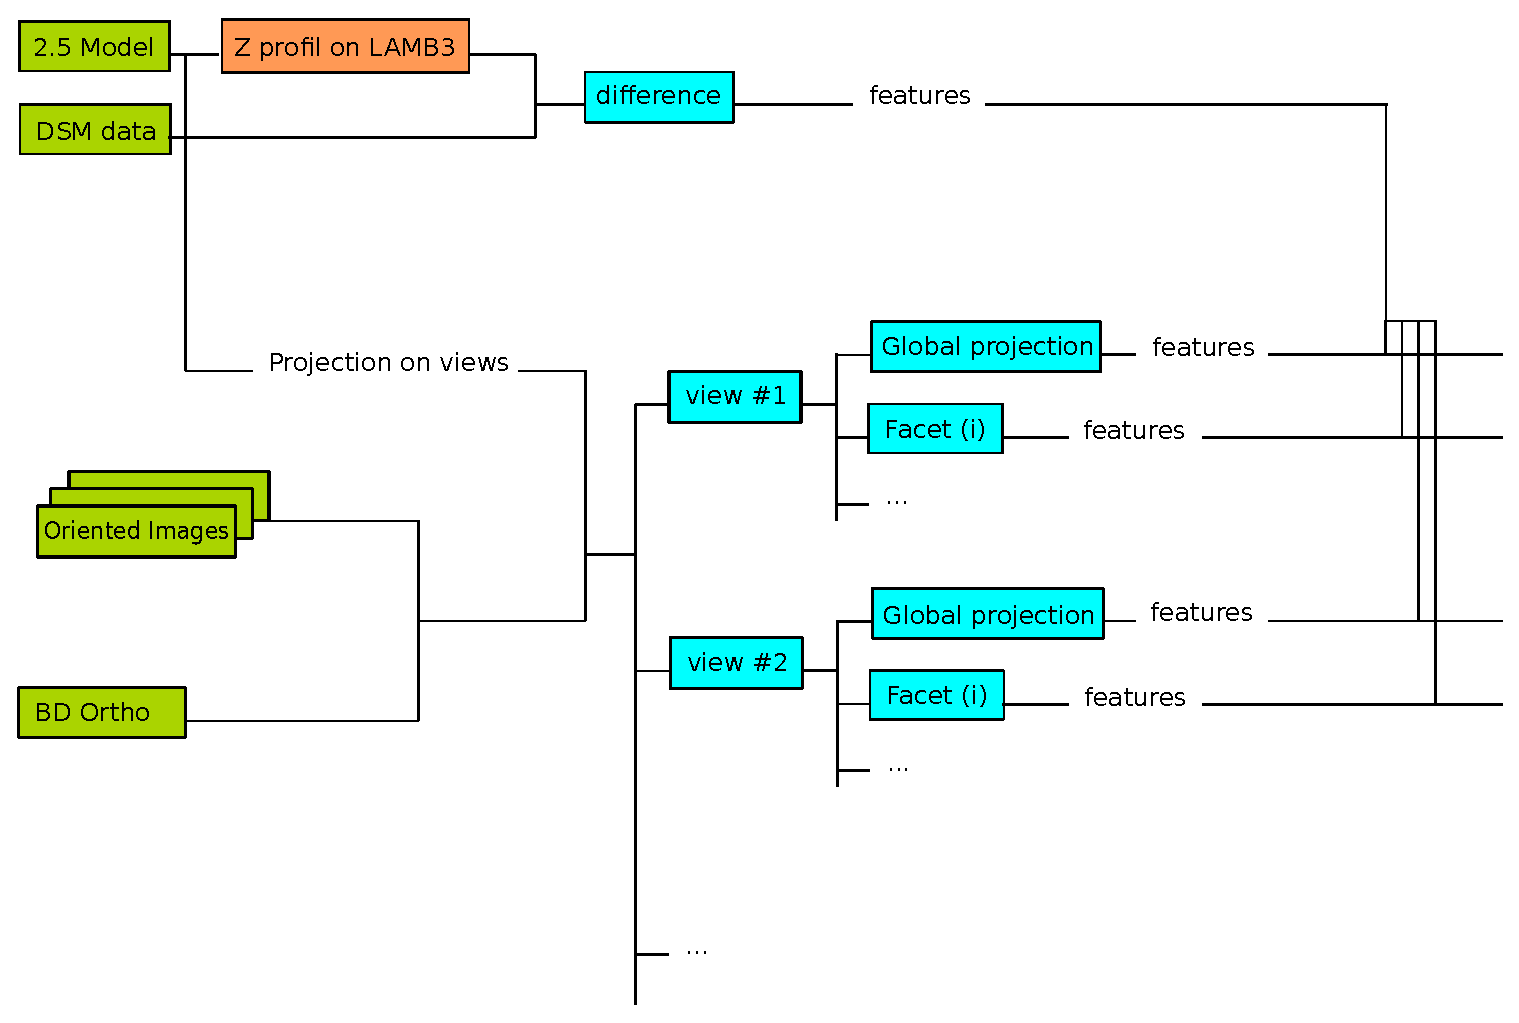
\includegraphics[scale=.5]{images/vectorial/pipeline.eps}
			\caption{Pipeline proposition.}
			\label{fig::pipeline}
		\end{center}
	\end{figure}
	
	In the feature extraction part, we can:
	\begin{itemize}
		\item look for very specific patterns behind the classified erros:
			\begin{itemize}
				\item[-] Chimneys,
				\item[-] Vegetation and building proximity,
				\item[-] Adjacent buildings,
				\item[-] Complex primitives,
				\item[-] Shades,
				\item[-] Gargoyles and dormer windows;
			\end{itemize}
		\item and/or, look for features charecterizing each error or a couple of errors:
			\begin{itemize}
				\item[-] Local errors: for each facet we try to compare it to the ground truth: segmentation errors. We can use superpixels \cite{Achanta:2012:SSC:2377349.2377556} and convex polygon segmentation \cite{duan2015image}.
				\item[-] Global roof errors: we construct the graph of adjacency of each facet and compare it to ground truth: DPM \cite{felzenszwalb2010object}, RJMCMC initialized with current faces or Edge detector + junction point process \cite{chai2013recovering}.
				\item[-] Dictionnary learning and easier Pooling \cite{bach2010sparse}.
				\item[-] Segmentation Error Detection on (MNS - Z profil).
			\end{itemize}
	\end{itemize}
	
	\section*{Results:}
	There is no results to report for now.
	
	\section*{Attachments:}
	
	You can checkout the Code in \href{https://github.com/Ethiy/3DSceneModel}{Github}.
	
	\bibliographystyle{alpha}
	\bibliography{references.bib}

\end{document}
